\documentclass{beamer}

\usepackage[utf8]{inputenc}
\usepackage[english]{babel}
\usepackage{textpos}
\usepackage{graphicx}
\usepackage{textcomp}
\usepackage{animate}
\usepackage{comment}
%\usepackage{multicol}
%\setlength{\columnsep}{5cm}
\usepackage{amsmath}
\usepackage{amsfonts}
\usepackage{verbatim}
\usepackage{varwidth}
\usepackage{caption}
\usepackage{dcolumn}
\usepackage{amssymb}
\usepackage{algorithm}
\usepackage{algorithmic}
%\usepackage{physics}
\usepackage{hyperref}
\usepackage{scalerel,stackengine}
\usepackage{fancyvrb}


\newcommand{\code}[1]{\texttt{#1}}
\newcommand{\shp}{$>>>$ }
\newcommand{\tab}{\hspace*{22pt}}

\usetheme{Madrid}

\title{Chapter 5: \\ Structured (Non-Scalar) Data Types}
\author{EEC 3150}
\date{}

\institute{Trevecca Nazarene University}
 


%%%%%%%%% BEGIN DOCUMENT %%%%%%%%%
%%%%%%%%% BEGIN DOCUMENT %%%%%%%%%
%%%%%%%%% BEGIN DOCUMENT %%%%%%%%%

\begin{document}

% get title page 
\frame{\titlepage}
 
%%%%%%%%%%
%%%%%%%%%%
\begin{frame}	
	\frametitle{Outline}
	\tableofcontents	
\end{frame}


%%%%%%%%%%
%%%%%%%%%%
\section{Tuples}

\begin{frame}	
	\center{\Huge{Tuples}}
\end{frame}

\begin{frame}	
	\frametitle{Tuples}
	
	\begin{alertblock}{Structured and unstructured data types:}
		\textbf{Unstructured data types} (or scalar dtypes) are objects which have no internal structure (they represent one piece of information)
		\begin{itemize}
			\item Examples: int, float, bool
		\end{itemize}
		\textbf{Structured data types} (or non-scalar dtypes) are objects which do have some kind of internal structure (they can represent multiple pieces of information)
		\begin{itemize}
			\item Examples we've seen already: string, range, tuple
			\item New examples: lists, dictionaries, sets
		\end{itemize}
	\end{alertblock}
	
\end{frame}

\begin{frame}	
	\frametitle{Tuples}
	
	\begin{alertblock}{Defn: tuples}
		\textbf{Tuple}: an ordered, immutable sequence of data elements
		
		\vspace{10pt}
		Rules:
		\begin{itemize}
			\item Parentheses, comma-separated
			\item Index/slice with square brackets (just like strings)
		\end{itemize}
		
		\vspace{10pt}
		Examples:
		\begin{itemize}
			\item \code{x = (1,)} (singletons require trailing comma)
			\item \code{x = (1,2,3)}
			\item \code{x = ()} (empty tuple)
			\item \code{x = (1, 'cow', True)} (multiple data types allowed)
			\item \code{x[0]} (index the 0th element of a tuple, like strings)
			\item \code{x = ( (1,2), (3,4) )} (tuple of tuples)
		\end{itemize}
	\end{alertblock}
	
\end{frame}

\begin{frame}	
	\frametitle{Tuples}
	
	\begin{block}{Tuples in action:}
		Operations on tuples:
		\begin{itemize}
			\item Concatenation: + (like strings)
			\item Repetition: * (like strings)
			\item Length: \code{len()} function
			\item Casting: \code{tuple()}
		\end{itemize}
		
		\vspace{10pt}
		Uses:
		\begin{itemize}
			\item Multiple arguments to a function
			\item Multiple returns from a function
			\item Shape of multi-dimensional numpy arrays (more on that later)
			\item Iterable with a for loop
		\end{itemize}
	\end{block}
	
\end{frame}


%%%%%%%%%%
%%%%%%%%%%
\section{Lists and Mutability}

\begin{frame}	
	\center{\Huge{Lists and Mutability}}
\end{frame}

\begin{frame}	
	\frametitle{Lists}
	
	\begin{alertblock}{Defn: lists}
		\textbf{List}: an ordered, mutable sequence of data elements
		
		\vspace{10pt}
		Rules:
		\begin{itemize}
			\item Square brackets, comma-separated
			\item Index/slice with square brackets (just like strings)
		\end{itemize}
		
		\vspace{10pt}
		Examples:
		\begin{itemize}
			\item \code{x = [1]} (singletons don't need comma)
			\item \code{x = [1,2,3]}
			\item \code{x = []} (empty list)
			\item \code{x = [1, 'cow', True]} (multiple data types allowed)
			\item \code{x[0]} (index the 0th element of a list, like strings)
			\item \code{x = [ [1,2], [3,4] ]} (list of lists)
		\end{itemize}
	\end{alertblock}
	
\end{frame}

\begin{frame}	
	\frametitle{Lists}
	
	\begin{block}{Lists in action:}
		Operations on lists:
		\begin{itemize}
			\item Concatenation: + (like strings)
			\item Repetition: * (like strings)
			\item Length: \code{len()} function
			\item Casting: \code{list()}
		\end{itemize}
		
		\vspace{10pt}
		Uses:
		\begin{itemize}
			\item Used infinitely more than tuples
			\item Let's talk about mutability first
		\end{itemize}
	\end{block}
	
\end{frame}

\begin{frame}%[fragile]
	\frametitle{Mutability}
	
	\begin{block}{Let's compare these codes:}
		\begin{itemize}
			\item These codes demonstrate defining a tuple/list \code{y} in terms of another \code{x} and then changing \code{x} afterwards
			\item In which codes does changing \code{x} change \code{y}? \\
					(\code{id()} returns an object's location in memory)
		\end{itemize}
		
		\vspace{10pt}
		\minipage{0.5\textwidth}
			\begin{footnotesize}
			\code{x = (1,) \\
			y = x \\
			print(y, x) \\
			print( id(y), id(x) ) \\
			\tab \\
			x = (1,2) \\
			\# x += (2,) \\
			\tab \\
			print(y, x) \\
			print( id(y), id(x) )
			}
			\end{footnotesize}
		\endminipage\hfill
		\minipage{0.5\textwidth}
			\begin{footnotesize}
			\code{x = [1] \\
			y = x \\
			print(y, x) \\
			print( id(y), id(x) ) \\
			\tab \\
			x = [1,2] \\
			\# x += [2] \\
			\# x.append(2) \\
			print(y, x) \\
			print( id(y), id(x) )
			}
			\end{footnotesize}
		\endminipage\hfill
	\end{block}
	
\end{frame}

\begin{frame}%[fragile]
	\frametitle{Mutability}
		
	\minipage{0.5\textwidth}
		\begin{figure}[ht]
			\centering
			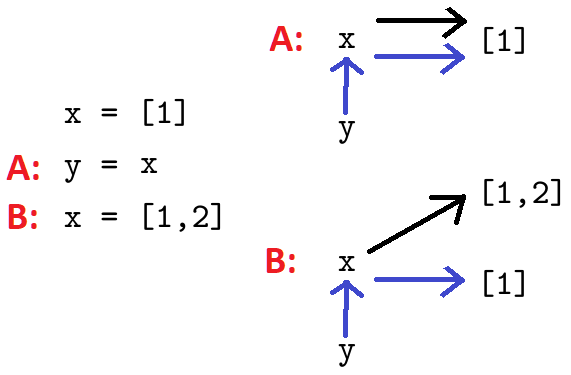
\includegraphics[width=0.9\linewidth]{Mutability_01}
%			\caption{Visual depiction of the algorithm}
		\end{figure}
		\begin{itemize}
			\item A: pass the current memory location of \code{x} to \code{y}
			\item B: change the contents of \code{x} \\
					(this method also changes it's location in memory)
			\item B: \code{y} still points to \code{x}'s old location, so it's unchanged
		\end{itemize}
	\endminipage\hfill
	\minipage{0.5\textwidth}
			\begin{figure}[ht]
			\centering
			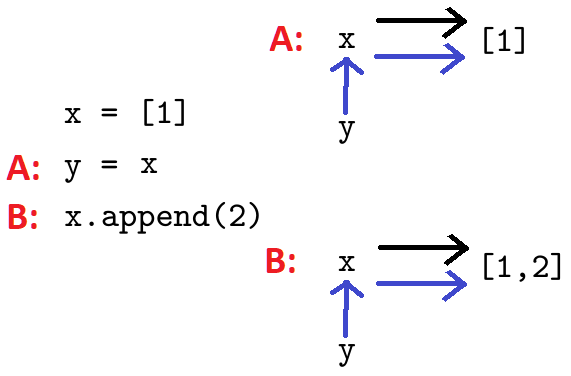
\includegraphics[width=0.9\linewidth]{Mutability_02}
%			\caption{Visual depiction of the algorithm}
		\end{figure}
		\begin{itemize}
			\item A: pass the current memory location of \code{x} to \code{y}
			\item B: change the contents of \code{x} \\
					(this method preserves it's location in memory)
			\item B: \code{x}, \code{y} still point to orig. locations, but with new values
		\end{itemize}
	\endminipage\hfill
	
\end{frame}

\begin{frame}	
	\frametitle{Mutability}
	
	\begin{alertblock}{Defn: mutability}
		\textbf{Mutable} objects in Python (and other languages) can be altered after being defined (opposite: immutable)
		
		\vspace{7pt}
		Consequences:
		\begin{itemize}
			\item Convenient for manipulating data (MANY cool functions)
			\item User-defined functions can alter global mutable objects WITHOUT the global keyword (show example code)
			\item Possible to unintentionally alter objects when defining them in terms of each other or copying (like the previous example)
			\item Solution: deep copy instead of shallow copy
		\end{itemize}
		
%		\vspace{10pt}
		Examples:
		\begin{itemize}
			\item Mutable: lists, dictionaries, sets
			\item Immutable: ints, floats, bools, strings, ranges, tuples, numpy arrays, pandas dataframes/series
		\end{itemize}
	\end{alertblock}
	
\end{frame}

\begin{frame}%[fragile]
	\frametitle{Lists}
	
	\begin{block}{List methods:}
		\begin{itemize}
			\item \textbf{Methods} are functions that are defined for only certain types of objects
			\item They are called using \emph{dot notation}: \\
					\code{x = [1] \\
					x.append(2)}
			\item Go to this link to see Python's list methods: \href{https://docs.python.org/3/tutorial/datastructures.html}{LINK}
			\item Examples in my Python example scripts
		\end{itemize}
	\end{block}
	
\end{frame}

\begin{frame}%[fragile]
	\frametitle{Lists}

	\minipage{0.48\textwidth}
		\begin{block}{Iterables:}
			Lists are \textbf{iterable}:
			\begin{itemize}
				\item Their elements can be returned one at a time and utilized in a for loop
			\end{itemize}
			
			\vspace{10pt}
			\code{x = [1, `cow', True] \\
			for i in x: \\
			\tab print(x)
			}
		\end{block}	
	\endminipage\hfill
	\minipage{0.04\textwidth}
	\endminipage\hfill	
	\minipage{0.48\textwidth}
		\begin{block}{Building lists with a loop and append:}
			Lists are often constructed in this format:
			\begin{itemize}
				\item Start with an initial list (usually empty)
				\item Append in a loop
			\end{itemize}
			
			\vspace{10pt}
			\code{x = [] \\
			for i in range(10): \\
			\tab if i\%2 == 0: \\
			\tab \tab x.append(i)
			}
		\end{block}
	\endminipage\hfill
	
\end{frame}

\begin{frame}%[fragile]
	\frametitle{Lists}
	
	\begin{block}{Some simple list programs:}
		\minipage{0.5\textwidth}
			Write a function which squares all \\ the elements of a list:
			
			\vspace{10pt}
			\code{def SquareList(x): \\
			\tab y = [] \\
			\tab for i in x: \\
			\tab \tab y.append(i**2) \\
			\tab \# end \\
			\tab return y
			}
		\endminipage\hfill
		\minipage{0.5\textwidth}
			Write a function which will concatenate a list of strings into one string with spaces in between them (no trailing whitespace):
			
			\vspace{10pt}
			\code{def ConcatStrings(x): \\
			\tab y = x[0] \\
			\tab for s in x[1:]: \\
			\tab \tab y += ` ' \\
			\tab \tab y += s \\
			\tab \# end \\
			\tab return y
			}
		\endminipage\hfill
	\end{block}
	
\end{frame}

\begin{frame}%[fragile]
	\frametitle{Lists}
	
	\begin{block}{Iterate through multiple lists: \code{zip()} and \code{enumerate()}:}
		\minipage{0.5\textwidth}
			Use \code{zip()} to iterate through \\ multiple lists at once:
			
			\vspace{10pt}
			\code{x = [1,2,3] \\
			y = [4,5,6] \\
			for i,j in zip(x,y): \\
			\tab print(i,j)
			}
			
			\vspace{10pt}
			\begin{itemize}
				\item If lists are different lengths, it goes the length of the shorter one
			\end{itemize}
		\endminipage\hfill
		\minipage{0.5\textwidth}
			Use \code{enumerate()} to iterate a list AND and its indices:
			
			\vspace{10pt}
			\code{y = [4,5,6] \\
			for i,j in enumerate(y): \\
			\tab print(i,j)
			}
			
			\vspace{10pt}
			\begin{itemize}
				\item Useful when you want to iterate a list without indexing a constantly but you also want the indices
			\end{itemize}
		\endminipage\hfill
	\end{block}
	
\end{frame}

\begin{frame}%[fragile]
	\frametitle{Lists}
	
	\begin{block}{Applying a function to list elements: \code{map()}}
		\begin{itemize}
			\item The \code{map(f,iter)} function applies the function \code{f} to each element in the iterable \code{iter} (list, tuple, etc.)
			\item It returns a \code{map} object which is useless so cast the result to the desired iterable at the end
		\end{itemize}
		
		\vspace{10pt}
		\minipage{0.5\textwidth}
			\code{def square(n): \\
					\tab return n**2 \\
					\# end \\
					x = [1,2,3] \\
					y = list(map(square,x)) \\
					print(y) 
					}
		\endminipage\hfill
		\minipage{0.5\textwidth}
			You can use \code{map()} to cast the elements of a list in one line:
			
			\vspace{10pt}
			\code{x = [1,2,3] \\
					y = list(map(str,x)) \\
					print(y) 
					}
		\endminipage\hfill
	\end{block}
	
\end{frame}

\begin{frame}%[fragile]
	\frametitle{Lists}
	
	\begin{exampleblock}{Primes:}
		Write a function which generates a list of the first $n$ primes. \\
		Be efficient: we only need to check if a number is divisible by any primes.
	\end{exampleblock}
	
\end{frame}

\begin{frame}
	\frametitle{Lists}
	
	\begin{block}{Nested lists:}
		It is very common in Python to make a list of lists:
		
		\vspace{10pt}
		\minipage{0.5\textwidth}
			\code{\shp x = [ [1,2], [3,4] ] \\
			\shp x[0] \\ \hspace{0pt}
			[1,2] \\
			\shp x[0][0] \\
			1 \\
			\shp x[1] \\ \hspace{0pt}
			[3,4] \\
			\shp x[1][1] \\
			4
			}
		\endminipage\hfill
		\minipage{0.5\textwidth}
			\begin{itemize}
				\item To access the inner-most items of a nested list, you must index the list multiple times
				\item The first level of indexing returns one of the lists
				\item The second will then index THAT list
			\end{itemize}
		\endminipage\hfill
		
		\vspace{15pt}
		Terminology:
		\begin{itemize}
			\item 2D list: list of lists
			\item 3D list: list of lists of lists
		\end{itemize}
	\end{block}
\end{frame}

\begin{frame}
	\frametitle{Lists}
	
	\begin{block}{Creating nested lists:}
		We can use nested loops to create/index nested lists:
		
		\vspace{10pt}
		\minipage{0.5\textwidth}
			\code{x = [] \\
			for i in range(n): \\
			\tab x.append([]) \\
			\tab for j in range(n): \\
			\tab \tab x[i].append( stuff ) 
			}
		\endminipage\hfill
		\minipage{0.5\textwidth}
			\begin{itemize}
				\item Start with an empty list \code{x}
				\item Outer loop: append empty lists to \code{x}
				\item Inner loop: append to the elements of \code{x} (which are themselves lists)
			\end{itemize}
		\endminipage\hfill
		
		\vspace{15pt}
		Terminology:
		\begin{itemize}
			\item Column: entries of a 2D list indexed vertically
			\item Row: entries of a 2D list indexed horizontally
		\end{itemize}
	\end{block}
	
\end{frame}

\begin{frame}
	\frametitle{Lists}
	
	\begin{block}{Row sum:}
		Write a function takes a 2D list and returns two lists: the row sums and column sums
		
		\vspace{10pt}
		\minipage{0.5\textwidth}
			\begin{footnotesize}
			\code{def RowColSum(x): \\[-5pt]
					\tab row = [] \\[-5pt]
					\tab for y in x: \\[-5pt]
					\tab \tab row.append(sum(y)) \\[-5pt]
					\tab \# end \\[-5pt]
					\tab \\[-5pt]
					\tab n = len(x) \\[-5pt]
					\tab m = len(x[0]) \\[-5pt]
					\tab col = [] \\[-5pt]
					\tab for i in range(n): \\[-5pt]
					\tab \tab col.append(0) \\[-5pt]
					\tab \tab for j in range(m): \\[-5pt]
					\tab \tab \tab col[i] += x[j][i] \\[-5pt]
					\tab \tab \# end \\[-5pt]
				\tab \# end \\[-5pt]
					\tab \\[-5pt]
				\tab return row, col \\[-5pt]
			\# end
			}
			\end{footnotesize}
		\endminipage\hfill
		\minipage{0.5\textwidth}
			\begin{itemize}
				\item Notice how much easier it is to get the row sums than the column sums
			\end{itemize}
		\endminipage\hfill
	\end{block}
	
\end{frame}

\begin{frame}%[fragile]
	\frametitle{Lists}
	
	\begin{exampleblock}{Identity matrix:}
		Write a function which generates an $n$-dimension identity matrix using a nested lists.
	\end{exampleblock}
	
	\begin{exampleblock}{Transpose:}
		Write a function which return the matrix transpose of a 2D list.
	\end{exampleblock}
	
\end{frame}


%%%%%%%%%%
%%%%%%%%%%
\section{Strings}

\begin{frame}	
	\center{\Huge{Strings}}
\end{frame}

\begin{frame}	
	\frametitle{Strings}
	
	\begin{block}{Strings revisited:}
		\textbf{String}: an ordered, immutable sequence of characters
		\begin{itemize}
			\item Go to this link to see Python's string methods: \href{https://docs.python.org/3/library/stdtypes.html?highlight=tuple\#string-methods}{LINK}
			\item Examples in my Python example scripts
		\end{itemize}
	\end{block}
	
	\begin{block}{ASCII:}
		\textbf{ASCII}: American Standard Code for Information Interchange
		\begin{itemize}
			\item All characters are stored as numbers
			\item An ASCII table shows these number/character conversion
			\item Conversion functions in Python: \\
					\code{\shp ord(`p') \\
					112 \\
					\shp chr(112) \\
					`p'
					}
		\end{itemize}
	\end{block}
	
\end{frame}

\begin{frame}%[fragile]
	\frametitle{Strings}
	
	\begin{figure}[ht]
		\centering
		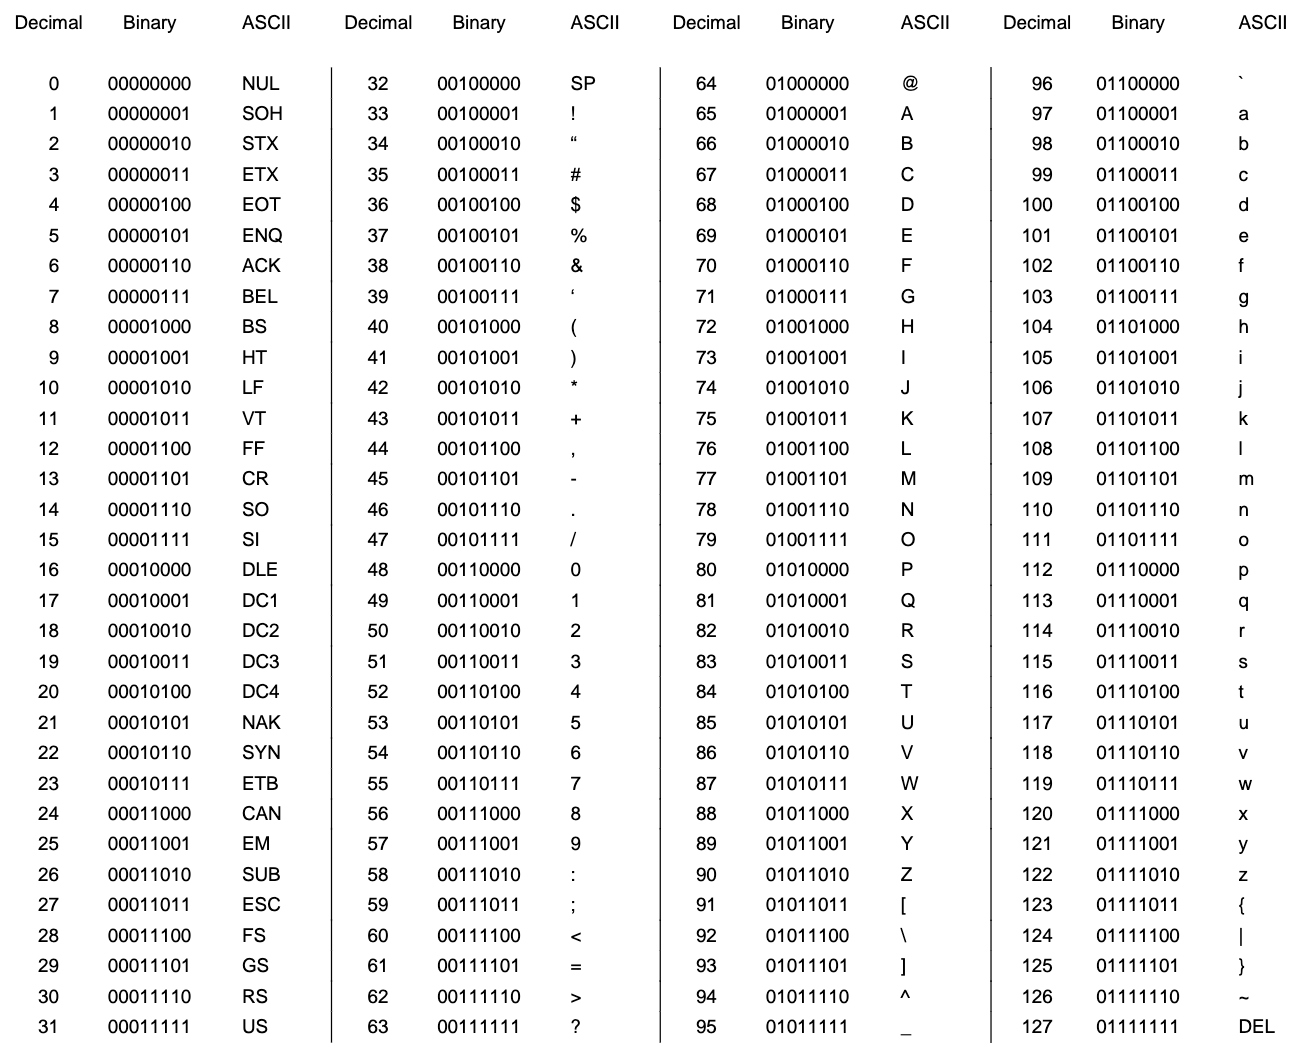
\includegraphics[width=0.8\linewidth]{ASCII}
%		\caption{Visual depiction of the algorithm}
	\end{figure}
	
\end{frame}

\begin{frame}	
	\frametitle{Strings}
	
	\begin{block}{More on strings:}
		\begin{itemize}
			\item Sorting a list of strings will sort them numerically via their ASCII codes
		\end{itemize}
	\end{block}
	
	\begin{block}{Escape characters:}
		An escape character utilizes a backslash (\textbackslash ) to use characters in strings that would otherwise be impossible or illegal to add:
		\begin{itemize}
			\item \textbackslash n: new line
			\item \textbackslash t: tab
			\item \textbackslash ': single quote
			\item \textbackslash '': double quote			
			\item \textbackslash\textbackslash : backslash
		\end{itemize}
	\end{block}
	
\end{frame}

\begin{frame}	
	\frametitle{Strings}
	
	\begin{exampleblock}{See dictionaries:}
		Our in-class exercise for strings will also use dictionaries. Look for it in the next section.
	\end{exampleblock}
	
\end{frame}


%%%%%%%%%%
%%%%%%%%%%
\section{Dictionaries}

\begin{frame}	
	\center{\Huge{Dictionaries}}
\end{frame}

\begin{frame}	
	\frametitle{Dictionaries}
	
	\begin{alertblock}{Defn: dictionaries}
		\textbf{Dictionaries}: an ordered (as of 3.7), mutable sequence of data elements (values) which are indexed with arbitrary labels (keys)
		
		\vspace{10pt}
		Rules:
		\begin{itemize}
			\item Curly brackets, comma-separated
			\item Index/slice with square brackets (just like strings)
			\item Access a \emph{value} by indexing with a \emph{key}
		\end{itemize}
		
		\vspace{10pt}
		Examples:
		\begin{itemize}
			\item \code{x = \{ 'a':1, `b':2, 'c':3, 1234:True\}} ( key:value )
			\item \code{\shp x[`a'] \\
							1 \\
							\shp x[1234] \\
							True
							}
		\end{itemize}
	\end{alertblock}
	
\end{frame}

\begin{frame}	
	\frametitle{Dictionaries}
	
	\begin{block}{Building dictionaries:}
		\minipage{0.5\textwidth}
			\code{x = \{ \} \\
			x[`a'] = 1 \\
			x[5] = `hello'
			}
		\endminipage\hfill
		\minipage{0.5\textwidth}
			\begin{itemize}
				\item You can build dictionaries by appending to an empty dictionary via indexing
			\end{itemize}
		\endminipage\hfill
	\end{block}
	
	\begin{block}{A common application for dictionaries:}
		\minipage{0.6\textwidth}
			\code{person = \{ \\
			`firstname':'Graham' \\
			`lastname':'West' \\
			`age':28 \\
			`employer':'TNU' \\
			`job':'instructor' \\
			`courses': [`EEC3150','INT0960'] \\
			\}
			}
		\endminipage\hfill
		\minipage{0.4\textwidth}
			\begin{itemize}
				\item You can use dictionaries as a database to store multiple kinds of data about one thing
			\end{itemize}
		\endminipage\hfill
	\end{block}

\end{frame}

\begin{frame}	
	\frametitle{Dictionaries}
	
	\begin{block}{Methods: \code{x.keys()} and \code{x.values()}}
		\minipage{0.6\textwidth}
			Here are two critical dictionary methods:
			
			\vspace{10pt}
			\code{\shp x = \{ 'a':1, `b':2, 'c':3 \} \\
			\shp x.keys() \\
			dict\_keys(['a', 'b', 'c']) \\
			\shp x.values() \\
			dict\_values([1, 2, 3])
			}
		\endminipage\hfill
		\minipage{0.4\textwidth}
			\begin{itemize}
				\item \code{x.keys()} will return the keys of \code{x}
				\item \code{x.values()} will return the values of \code{x}
				\item These aren't lists, but they are iterable
			\end{itemize}
		\endminipage\hfill
	\end{block}
	
	\begin{block}{Iterating over a dictionary with \code{x.items()}}
		\minipage{0.5\textwidth}
			\code{x = \{ 'a':1, `b':2, 'c':3 \} \\
			for k, v in x.items(): \\
			\tab print(k,v)
			}
		\endminipage\hfill
		\minipage{0.5\textwidth}
			\begin{itemize}
				\item The \code{x.items()} method allows you to iterate over key/values pairs
				\item There are more dictionary methods, but these are the most important
			\end{itemize}
		\endminipage\hfill
	\end{block}
	
\end{frame}


\begin{frame}%[fragile]
	\frametitle{Dictionaries}
	
	\begin{exampleblock}{String character counts:}
		\begin{itemize}
			\item Write functions which will return a dictionary containing the counts of every unique character/word in a string
			\item Ignore case in both functions
			\item In the word function, strip any whitespace or punctuation
			\item Print each in descending order
		\end{itemize}
	\end{exampleblock}
	
\end{frame}

%%%%%%%%%%
%%%%%%%%%%
\section{Sets}

\begin{frame}	
	\center{\Huge{Sets}}
\end{frame}







\begin{comment}


\begin{frame}%[fragile]
	\frametitle{Functions}
	
	\begin{block}{Example: bisection root}
		Let's now write our bisection root-finder as a function:
		
		\vspace{15pt}
		\minipage{0.5\textwidth}
			\begin{figure}[ht]
				\centering
				
\includegraphics[width=0.9\linewidth]{RootFunction}
%				\caption{Visual depiction of the algorithm}
			\end{figure}
		\endminipage\hfill
		\minipage{0.5\textwidth}
			\begin{itemize}
				\item Accepts 3 arguments:\\
						1. \code{x}: the number to be ``rooted'' \\
						2. \code{power}: the power of the root \\
						3. \code{epsilon}: the error tolerance
				\item Returns \code{None} if it can't compute the root
			\end{itemize}
		\endminipage\hfill
	\end{block}
	
\end{frame}


\end{comment}




\end{document}




